\section{Particles in the heliosphere}
\label{sec:particles_heliosphere}

Our heliosphere is a vast region in space embedded in the \ac{ISM}, which encompasses all solar system planets and extends far beyond even the Kuiper belt. 
It is filled with a thin plasma consisting of various populations of particles, many of which originate from the Sun itself. These populations can be seen in \autoref{fig:heliospheric_energy_spectrum} \citep[based on measurements by][]{Mewaldt-2001}, shown as an energy spectrum that extends over more than 7 orders of magnitude on the energy scale and about 20 orders of magnitude on the intensity scale.
The by far most abundant population is the solar wind, a steady flow of plasma that is emitted from the Sun radially and fills the heliosphere. 
In the near-Earth space at one astronomical unit (\si{\AU}), the slow solar wind reaches typical speeds between \SIrange[range-phrase={\,and\,}]{300}{500}{\kilo\meter\per\second}.
Due to its low pressure, and therefore high plasma $\beta$, it carries the solar magnetic field with it and forms the \ac{IMF}.
As the Sun rotates, the \ac{IMF} carried by the solar wind is forms an Archimedian spiral, which is named Parker spiral after Eugene N. \citet{Parker-1958}, who first developed this model of the solar wind.

\begin{figure}
    \centering
    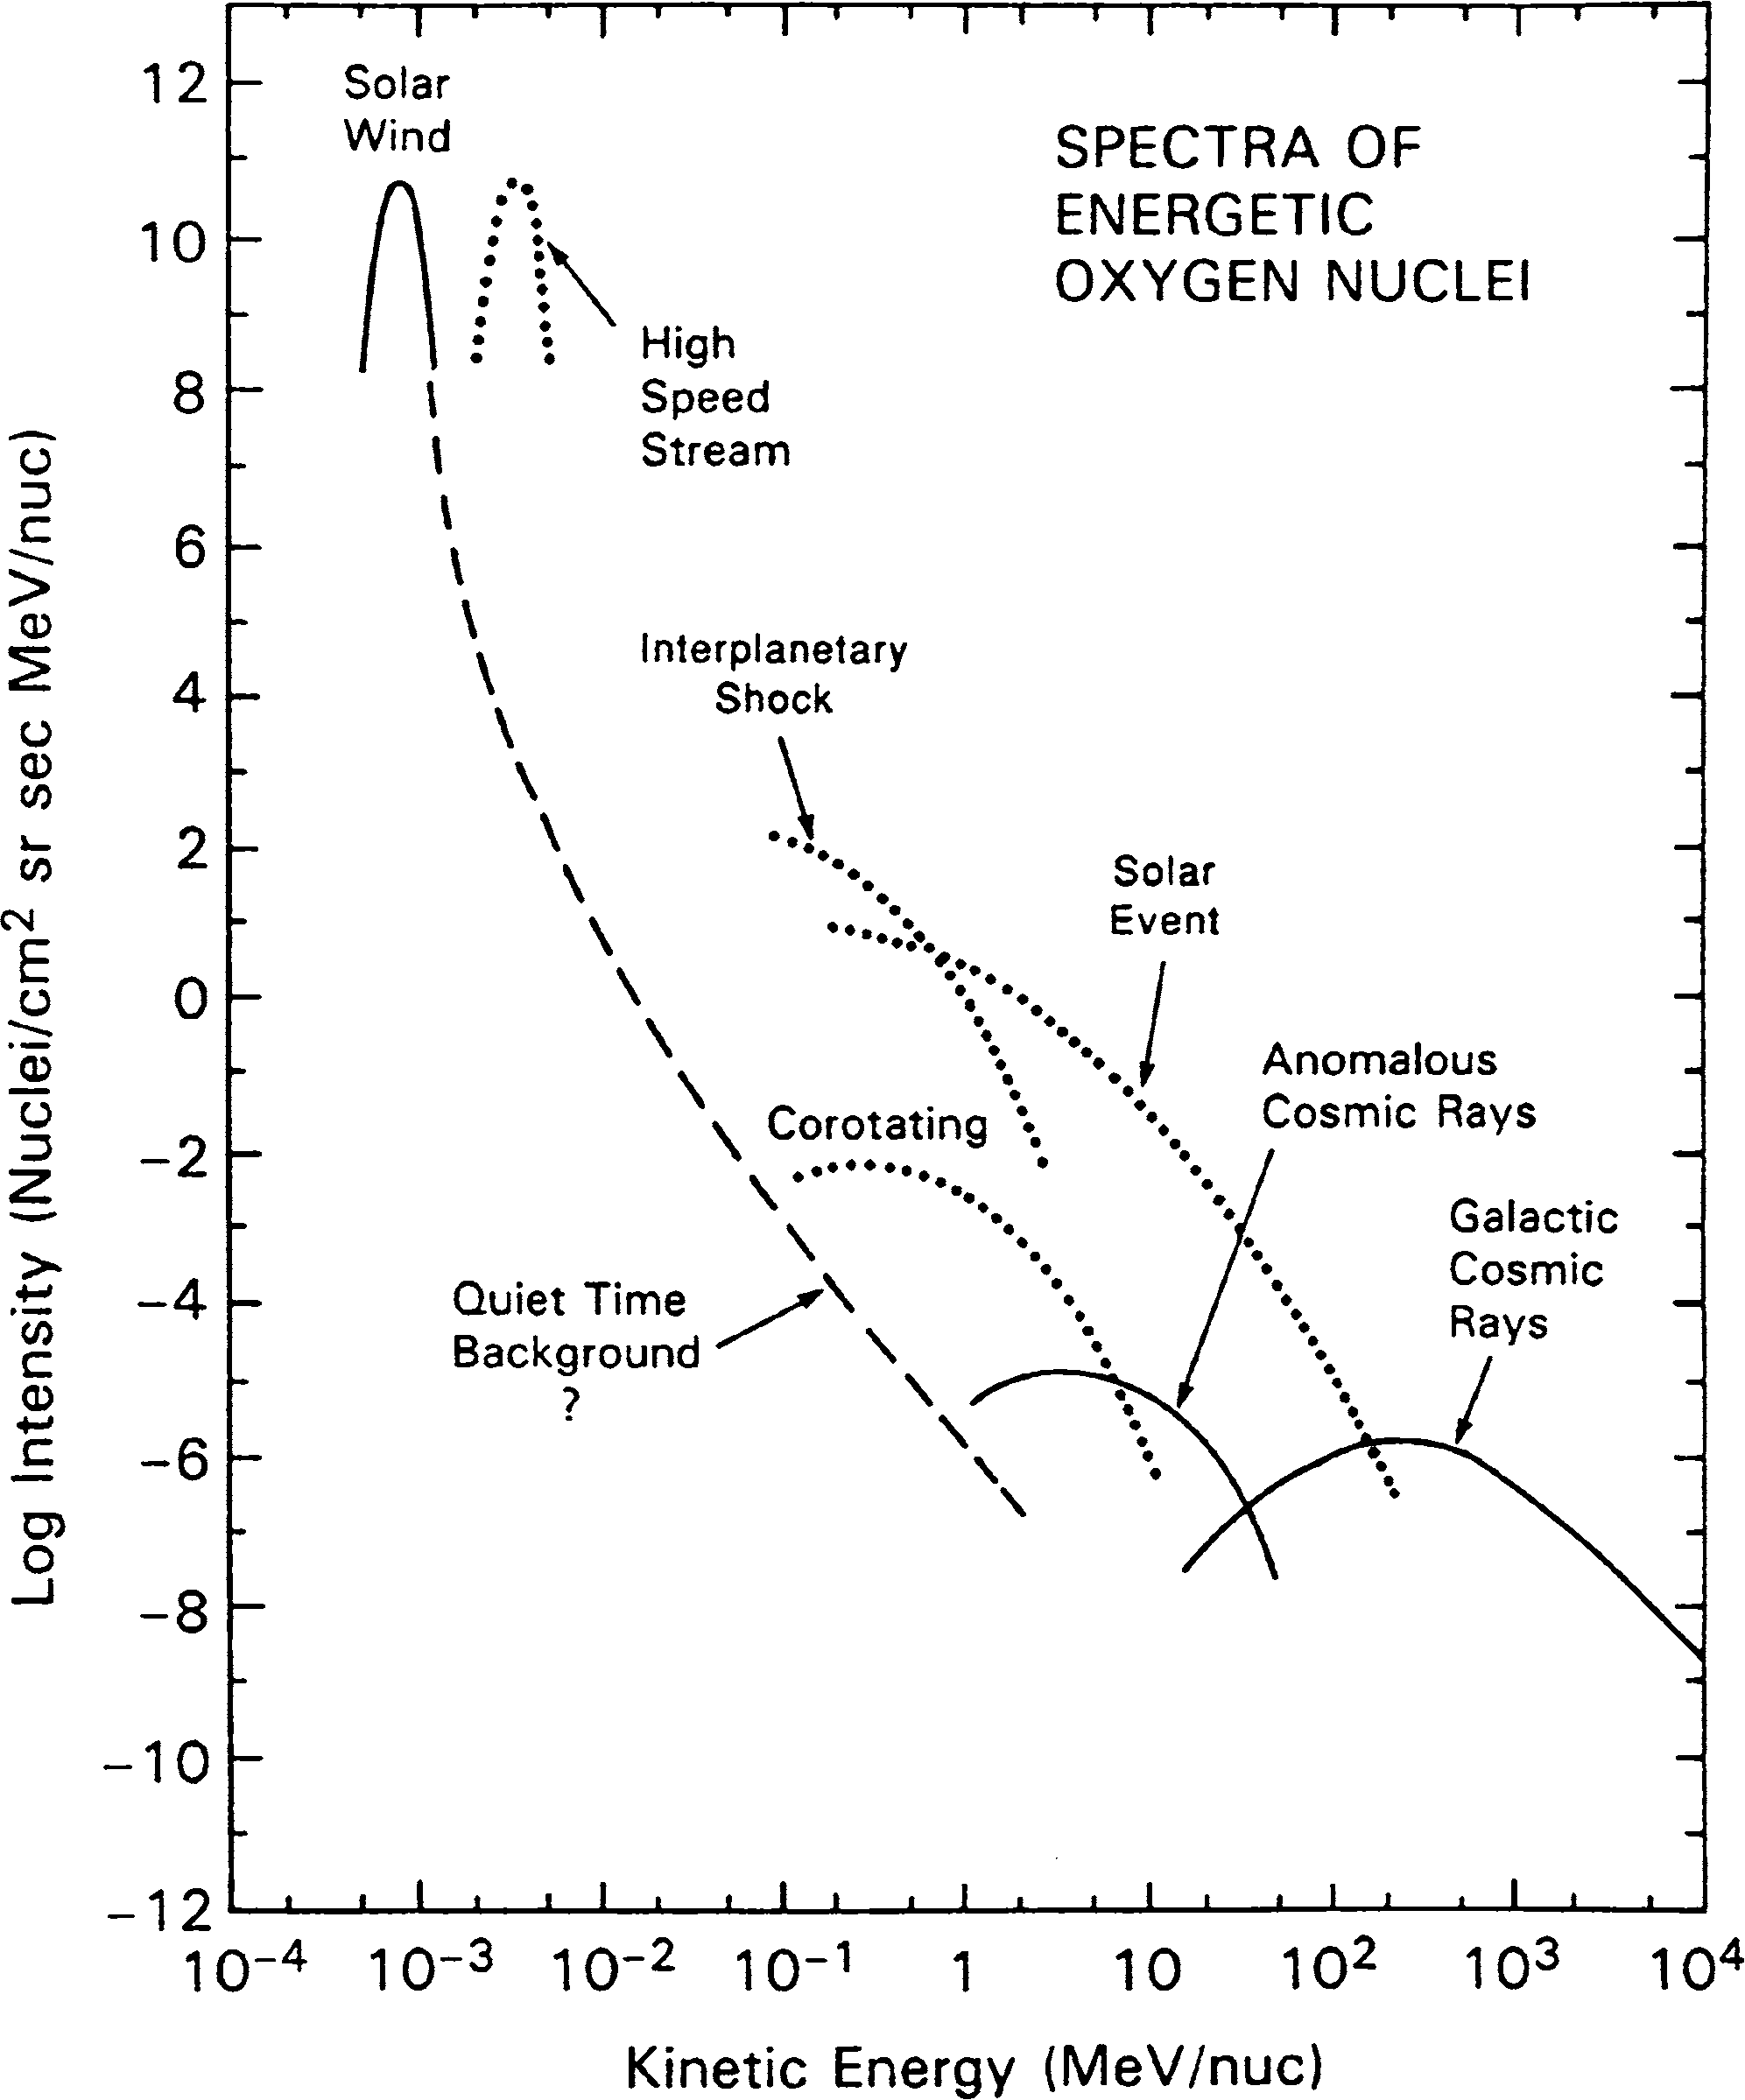
\includegraphics[width=0.6\linewidth]{images/heliospheric_energy_spectrum}
    \caption[Spectra of oxygen ions in the near-Earth interplanetary space]{Typical spectra of oxygen ions in the near-Earth interplanetary space, showing the contributions from different populations. Other particle species show similarly shaped spectra when plotted as a function of energy/nucleon. (adapted from \url{http://helios.gsfc.nasa.gov/ace/gallery.html}, based on \cite{Mewaldt-2001}).}
    \label{fig:heliospheric_energy_spectrum}
\end{figure}

However, our Sun is an active star, and thus, the flow of particles is not simply constant. The variability is driven by the 11-year solar cycle, a recurring reversal of the solar magnetic field that is associated with enhancements in solar activity (solar maxmimum) due to the increased amount of magnetic stress and reconnection processes, and low-activity periods (solar minimum) inbetween.
Coronal holes, colder and therefore darker regions forming on the Sun, emit faster solar wind streams with speeds $\gtrsim \SI{600}{\kilo\meter\per\second}$, which interact with the neighboring streams of slower wind due to their different Parker spiral curvature. These interacting streams then form a \acl{SIR}\acused{SIR} \citep[\acs{SIR}, e.g.][]{Richardson-2018}, which flanked by interplanetary shocks on each side, the so-called forward and reverse shocks. If a coronal hole stays stable for a longer time, these interaction regions can be observed recurrently in each solar rotation (i.e., every $\sim$27 days when observed from Earth), in which case they are called \acp{CIR}.
Furthermore, active regions on the Sun can occasionally produce solar flares, sudden and intense emissions of light often associated with the release of high-energy ($\sim \si{\mega\electronvolt}$) \aclp{SEP}\acused{SEP} \citep[\acsp{SEP}, e.g.][]{Reames-1990}.
These are believed to be powered by reconnection of magnetic field lines at the Sun, which leads to the release of energy and acceleration of particles.
They often also coincide with the eruption of plasma from the solar corona in the form of a \ac{CME} at speeds up to a few thousands of \si{\kilo\meter\per\second}.
Just like the solar wind, \acp{CME} carry a magnetic field with them, often in the form of a flux rope propagating away from the Sun. Due to their high speed, a shock can form in front of the flux rope, followed by a turbulent sheath region.
This shock can also be efficient at accelerating additional particles to higher energies, similar to \acp{SEP} particles accelerated directly at the Sun.

At the high end of the energy spectrum (\autoref{fig:heliospheric_energy_spectrum}), at \si{\mega\electronvolt} to  \si{\giga\electronvolt} energies, we find \acp{GCR}, charged particles originating from outside the heliosphere produced e.g. in stellar supernovae and entering it with a relatively constant and isotropic flux. 
The flux of these high-energy particles within the heliosphere is modulated by various effects: In the long term, the variation of the \ac{IMF} intensity during the 11-year solar cycle modulates the \ac{GCR} intensity observed in the inner solar system, so that the average \ac{GCR} flux is higher during solar minimum than at solar maximum \citep{Fisk-1980}. In addition, there are short-term modulations of \ac{GCR} due to magnetic structures in the solar wind, such as \acp{CME} and \acp{SIR}/\acp{CIR}. These are the so-called Forbush decreases, which will be the main focus of this thesis.

\section{Space Weather events and their detection}
\label{sec:spaceweather}

As defined by the U.S. National Space Weather Program \parencite{OFCM-1995}, the term \textit{space weather} refers to ``conditions on the Sun and in the solar wind, magnetosphere, ionosphere and thermosphere that can influence the performance and reliability of space-borne and ground-based technological systems and endanger human life or health''.
The aforementioned large-scale heliospheric events, such as \acp{SEP}, \acp{CME} and \acp{CIR} are all relevant to space weather researchers, as both the increased radiation exposure due to accelerated energetic particles as well as the magnetic field disturbances, which impact spacecraft or disturb the Earth's magnetosphere in a so-called geomagnetic storm, can have such impacts on technology or human life on Earth, in space, and on other planets.

Thus, the focus in space weather research is to enhance the understanding of these events in order to be able to more accurately predict their occurrence and propagation, including the onset time at Earth (or other locations in the solar system) and their intensity.
In the past, the investigation of these events has been mostly based on two kinds of measurements: Remote-sensing observations of the Sun and its vicinity made from near Earth, such as \ac{EUV} images, magnetograms and white-light coronagraph images available from spacecraft such as \acs{SOHO} and \acs{SDO}, as well as in situ observations at or near Earth, using plasma measurements and magnetometers on spacecraft orbiting Earth (e.g., IMP-8, GOES) or at the $L_1$ Lagrange point (\acs{ACE}, \acs{SOHO}, Wind, \acs{DSCOVR}).
In the last two decades, such observations have been complemented by in situ measurements from deep space heliophysics missions, such as from the two \ac{STEREO} spacecraft orbiting the Sun near \SI{1}{\AU} as well as the recent \ac{PSP} and \ac{SolO} missions, which are starting to provide valuable data from extremely close to the Sun with a larger variety of instruments and higher resolution than the Helios mission in the 1970s. Additionally these missions facilitate imaging observations from additional vantage points, and these do not only cover the Sun and the corona, but also observe a wide-angle view of the interplanetary space using their \acp{HI}, which can be used to directly track \acp{CME} all the way out to Earth (see \autoref{sec:stereohi}).

\section{CMEs and ICMEs}
\label{sec:cmes}

As mentioned in Section \ref{sec:particles_heliosphere}, \acp{CME} are large-scale eruptions of plasma from the Sun that propagate outward into the heliosphere, which are often associated with flares and believed to be driven by reconnection of the coronal magnetic field \citep[see e.g.][for discussions on the triggering mechanism]{Forbes-2000,Kusano-2012}. CMEs occur relatively frequently, on average approximately every 4 days at solar minimum, and 2.5 to 3 times per day at solar maximum \citep{Webb-1994}. The properties of CMEs have a large variability: E.g., their speeds can range between \SIrange[range-phrase={\,and\,}]{20}{2000}{\kilo\meter\per\second}, where the average is at about \SI{400}{\kilo\meter\per\second}, and faster CMEs are more likely to occur near solar maximum. The longitudinal extent can also differ, very narrow (\SI{5}{\degree}) and very wide (\SI{120}{\degree}) cases have been observed, with the average being around \SI{50}{\degree} \citep{Cane-2000}.

When the counterparts of \acp{CME} are observed in situ in interplanetary space, they are often referred to as an interplanetary \ac{CME} \acused{ICME}(\acs{ICME}). Common \ac{ICME} signatures include a low proton temperature and density, an enhanced and often smoothly rotating magnetic field (magnetic cloud), bidirectional electron streaming, as well as the modulation of some elemental abundance ratios \citep{Richardson-Cane-1995,Zurbuchen-2006-insitu-signatures,Wimmer-Schweingruber2006}
As a \ac{CME}'s magnetic ejecta is often propagating at a higher velocity than the surrounding solar wind plasma, a turbulent region of compressed plasma, called the sheath, typically forms in front of these \acp{CME}. Solar wind plasma in front can be accumulated into the sheath, causing it to grow over time, but lateral flow away from the CME apex and magnetic reconnection with the ejecta can counteract this \citep[see e.g.][]{Siscoe2008,Manchester2005,Janvier-2019}. When the \ac{CME} exceeds the local magnetosonic speed, a shock front forms in front of the sheath, which is then observed as an abrupt change in the most parameters that are measured in situ, such as the magnetic field, plasma velocity and density.
As it has become clear, especially since the availability of \ac{HI} observations, that the structures observed near the Sun and in interplanetary space are directly linked, the lines between the terms \ac{CME} and \ac{ICME} have become more blurred, and many authors have begun to use the term \ac{CME} for both the remote sensing and in situ phenomena.

Many efforts have been made to develop models that describe the propagation of \acp{CME} in the heliosphere and predict their arrival times at different locations, taking into account the interaction with the surrounding ambient solar wind and other interplanetary structures, such as \acp{SIR} and other \acp{CME}. Most of these models can be divided into two basic classes: \ac{MHD} simulations and empirical models. One of the most widely used \ac{MHD} models in this field is the Wang-Sheeley-Arge ENLIL with cone model (WSA-ENLIL+Cone) developed by \citet{Odstrcil-2004}. WSA-ENLIL simulates the solar wind propagation in the heliosphere based on magnetogram observations of the Sun and a potential field source surface model of the coronal magnetic field (WSA model) within \SI{21.5}{\solarradius}, which is then used as the inner boundary of the \ac{MHD} simulation (ENLIL). CMEs can be injected into the \ac{MHD} model as a dense cone-shaped hydrodynamic bubbles starting from the inner boundary at \SI{21.5}{\solarradius}.

As it has long been known that the strongest geomagnetic storms are typically caused by \acp{ICME} with a strong southward magnetic field \citep[negative $B_z$, see e.g.][]{Russell-1974}, it became clear that these simple density bubbles without an inherent magnetic field are not sufficient for predicting the in situ magnetic field.
Therefore, in the recent years, a new heliospheric \ac{MHD} model named \acl{EUHFORIA}\acused{EUHFORIA} \citep[\acs{EUHFORIA},][]{Pomoell-2018} has been developed, which initially used the same cone model for describing the \acp{CME}, but was later adapted with a new spheromak model \citep{Scolini-2019}, which includes the magnetic field of the \ac{CME} and thus has substantially improved the predictions of the magnetic field observations at Earth.

On the other hand, there are simple empirical models of CME propagation, such as the analytical \acl{DBM}\acused{DBM} \citep[\acs{DBM},][]{Vrsnak-2013}. The \ac{DBM} is used to predict the \ac{ICME} arrival time at different points in space, it does not provide any predictions of the solar wind plasma or magnetic field. It is based on the well-known effect that due to the interaction of \acp{CME} with the ambient solar wind, and the \ac{CME} velocity $v$ tends to approach the solar wind speed $w$ over time. In reality, these forces are not created by the actual collision of particles, but transported in the form of \ac{MHD} waves and turbulence generated in the plasma \citep[see e.g.][for details]{Cargill-1996,Owens-2004}. \ac{DBM} describes the acceleration $a$ of the \ac{CME} in the mathematical form of a simple aerodynamic drag equation with an empirical drag parameter $\gamma$:
\begin{equation}
    a = -\gamma (v-w) |v-w|
\end{equation}
The advantage of such a model is that its results are much quicker to calculate (e.g., in real time prediction environments) and requires less input parameters. It can also be employed in a reverse modeling approach, where the model is fitted to the observed arrival times to determine the drag parameter \citep{Zic-2015}. Furthermore, the analytical form and fast computation time of the model allow to easily propagate the uncertainties of the input parameters, either analytically or with an ensemble modeling technique (DBEM) as proposed by \citet{Dumbovic-2018}.

As has been shown in the statistical studies by \citet{Vrsnak-2014,Dumbovic-2018} and others referenced therein, it seems that all common modeling approaches, independent of their complexity, show a surprisingly similar performance when it comes to the prediction of arrival times, with a mean absolute error on the order of \SI{10}{\hour} for large samples of \acp{CME} arriving at Earth. Even other independent approaches, such as recent studies that successfully predicted arrival times using convolutional neural networks based on coronagraph images without any manual intervention to determine the input parameters \citep{Wang-2019} have not yet been able to significantly surpass this accuracy, which would be desirable for space weather forecasting purposes. This suggests that more measurements at different heliospheric locations will need to be incorporated into such models in the future --- both to provide additional input parameters from observations close to the Sun and to create a larger sample size of in situ data for better calibrating the models.

\section{Forbush decreases}
\label{sec:forbush}

\citet{Forbush-1937} and \citet{Hess-1937} first discovered short-term decreases in the \ac{GCR} intensity detected in ionization chambers, which were detected at multiple stations simultaneously and coincided with geomagnetic storms. These decreases, which are routinely detected today using ground-based neutron monitors or spaceborne energetic particle detectors, were later named \acp{FD} in honor of their discoverer. It was found that \acp{FD} are not caused by the geomagnetic field variations themselves (as they are even observed at the poles), but rather have an interplanetary origin \citep[see e.g.][and references therein]{Lockwood1971}. There are two types of \ac{FD}: The so-called recurrent decreases, which are caused by \acp{CIR} and therefore reoccur after one solar rotation ($\sim$27 days), and the non-recurrent decreases caused by \acp{CME}. In both cases, the turbulent magnetic field of the shocks and sheaths associated with \acp{CME} or \acp{CIR}, as well as the strong magnetic field of a \ac{CME} flux rope can act as a barrier for \acp{GCR}, so that the intensity is decreased during the passage of this structure.
Especially in the case of \acp{CME}, the decrease phase is usually short ($\lesssim$ 1 day), while the recovery to the previous \ac{GCR} intensity (in the case of isolated events) can take multiple days up to $\sim$ a week. The onset typically corresponds well with the arrival of the \ac{CME} or shock/sheath structure, and in the case of \acp{CME} driving a shock a two-step decrease can sometimes be observed, with the first step caused by the shock/sheath region and the second by the magnetic ejecta --- this classical picture is displayed in \autoref{fig:richardsoncane-cme}. However, when the resolution of the \ac{GCR} measurements is not high enough, the second step may not be clearly separable for all events associated with a shock.
\begin{figure}
	\centering
	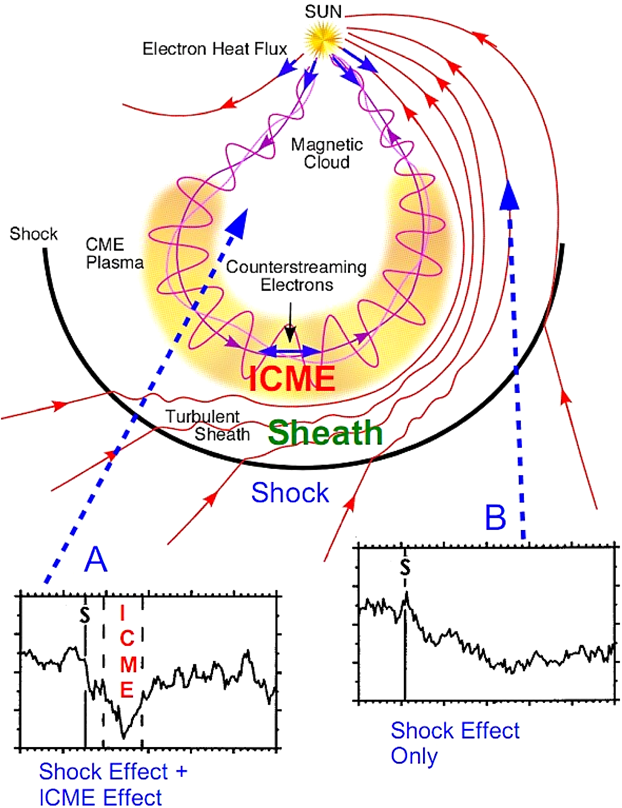
\includegraphics[width=0.6\textwidth]{images/richardson_cane_2011_icme.png}
	\caption{Illustration of an ICME that drives a shock and causes a classical two-step Forbush decrease at location A, where both the shock/sheath and the magnetic cloud pass. At location B, only a single-step Forbush decrease is observed because only the shock is seen here. Source: \citet[Figure 1]{Richardson-Cane-2011}, reprinted by permission from Springer Nature.}
	\label{fig:richardsoncane-cme}
\end{figure}
Typical amplitudes of \acp{FD} can range from a few percent up to more than \SI{10}{\percent} depending on the event, but this varies significantly depending on which particle energies are observed, as lower energy particles are modulated more easily and thus show larger \acp{FD} \citep[e.g.][]{Lockwood1971,Lockwood1991}.

Models have been proposed to describe the \acp{FD} caused by different magnetic structures, and these are often based on a diffusion equation. For example, the \acl{PDB}\acused{PDB} model \citep[\acs{PDB},][]{Wibberenz-1998} can be used to describe a shock acting as a barrier through which \acp{GCR} cannot diffuse as easily as in the ambient solar wind. This causes a ``shadow'' within and behind the barrier in which the \ac{GCR} intensity is decreased.
The \ac{ForbMod} developed by \citet{Dumbovic2018-ForbMod} builds on top of this approach to model \acp{FD} caused by flux rope \acp{CME} by combining the diffusion process with an expanding cylindrical flux rope structure. In this case, the flux rope initially does not contain any \acp{GCR} close to the Sun and the time evolution of the \ac{GCR} density within the flux rope is determined by the interplay of its self-similar expansion and the diffusion of \acp{GCR} into it. In a following article, \citet{Dumbovic-2020-ForbMod}, the model was combined with empirical equations for the energy dependence of the \ac{FD}, so that \acp{FD} measured by different instruments can be modeled taking into account their response functions. \ac{ForbMod} has been applied in two of the publications included in this PhD thesis \citep{Forstner-2020,Forstner-2021-SolO} and further details about its derivation are given in these publications.

\section{Motivation}
\label{sec:motivation}

To better understand the propagation of \acp{ICME} in the heliosphere, their radial evolution and impacts on Earth, it is essential to make measurements not only in situ at Earth, but from as many locations as possible, to be able to validate and calibrate modeling approaches and thus improve our forecasting capabilities. This includes both in situ measurements at different locations on the \ac{ICME}'s trajectory, e.g. as an upstream monitor to give early warning of an approaching \ac{ICME}, as well as remote sensing observations from the side to better understand the global \ac{CME} characteristics. Measurements at other locations also become increasingly relevant for the large amount of operating and planned space missions (including e.g. human spaceflight to Mars in the next decades), which are also in need of space weather forecasting for safe operations.

While spacecraft with appropriate plasma and magnetic field measurements are available at some locations, it is also sensible to introduce \acp{FD} into the framework of space weather observations, as some missions only carry particle detectors or provide other data only in limited form. For example, the \ac{RAD} instrument on the \ac{MSL} mission, which will be introduced in \autoref{sec:mslrad}, has been and still is the only instrument that provides continuous coverage of space weather at Mars through its \ac{FD} observations --- other missions such as Mars Express (2003) and MAVEN (2014) carry some plasma or magnetic field instruments, but only have limited coverage as their orbits dip into the bow shock of Mars so that the upstream solar wind cannot be observed all the time. This thesis will present the first systematical studies of Forbush decreases at Mars using the \ac{RAD} cosmic ray data and use the measured \ac{CME} arrival times as well as remote sensing data from \ac{STEREO}-\ac{HI} to validate different modeling approaches. Furthermore, it will be explored whether it is possible to derive more information about the \ac{CME} evolution than just the arrival times from the \ac{FD} observations by applying reverse modeling approaches, and case studies of some notable space weather events will be conducted.

In \autoref{chp:instruments}, a detailed overview of the most important instruments employed in these studies and their data products will be given. The following chapters present several peer-reviewed publications that study \ac{ICME} arrival times at \SI{1}{\AU} and Mars using \acp{FD} and remote sensing observations (\autoref{chp:arrival_times}), additional properties of \acp{FD} at Earth and Mars and their implications for \ac{CME} radial evolution (\autoref{chp:fd_properties}) as well as case studies of a major \ac{SEP} event at Mars that was associated with multiple \acp{ICME} (\autoref{chp:september_event}) and of the first \ac{ICME} and the corresponding \ac{FD} observed at the Solar Orbiter spacecraft (\autoref{chp:solo}). Three appendices follow, which describe certain technical aspects of these studies in more detail, such as the derivation of response functions for the \ac{HET} onboard Solar Orbiter (\autoref{chp:HETSimulation}) and the development of a new software tool implementing of the \ac{GCS} model for the reconstruction of \acp{CME} in remote sensing observations (\autoref{chp:GCS_Python}). Finally \autoref{chp:Publicationlist} presents a list of all publications that I have contributed to, including those that are not included within this PhD thesis as they do not directly fit into the logical flow.
